
\section{Object Reconstruction}
\label{sec:cmsExperiment:reconstruction}

% overview
The structure design of the CMS detector is ideal for the particle-flow reconstruction, which uses information from all subdetector systems to reconstruct each of the final state particles, including muons, electrons, photons, and hadrons. Based on the reconstructed particles, also known as the particle-flow candidates, jets are computed and then tagged by the \PQb jet tagger and hadronic tau tagger.

\begin{figure}[ht]
    \centering
    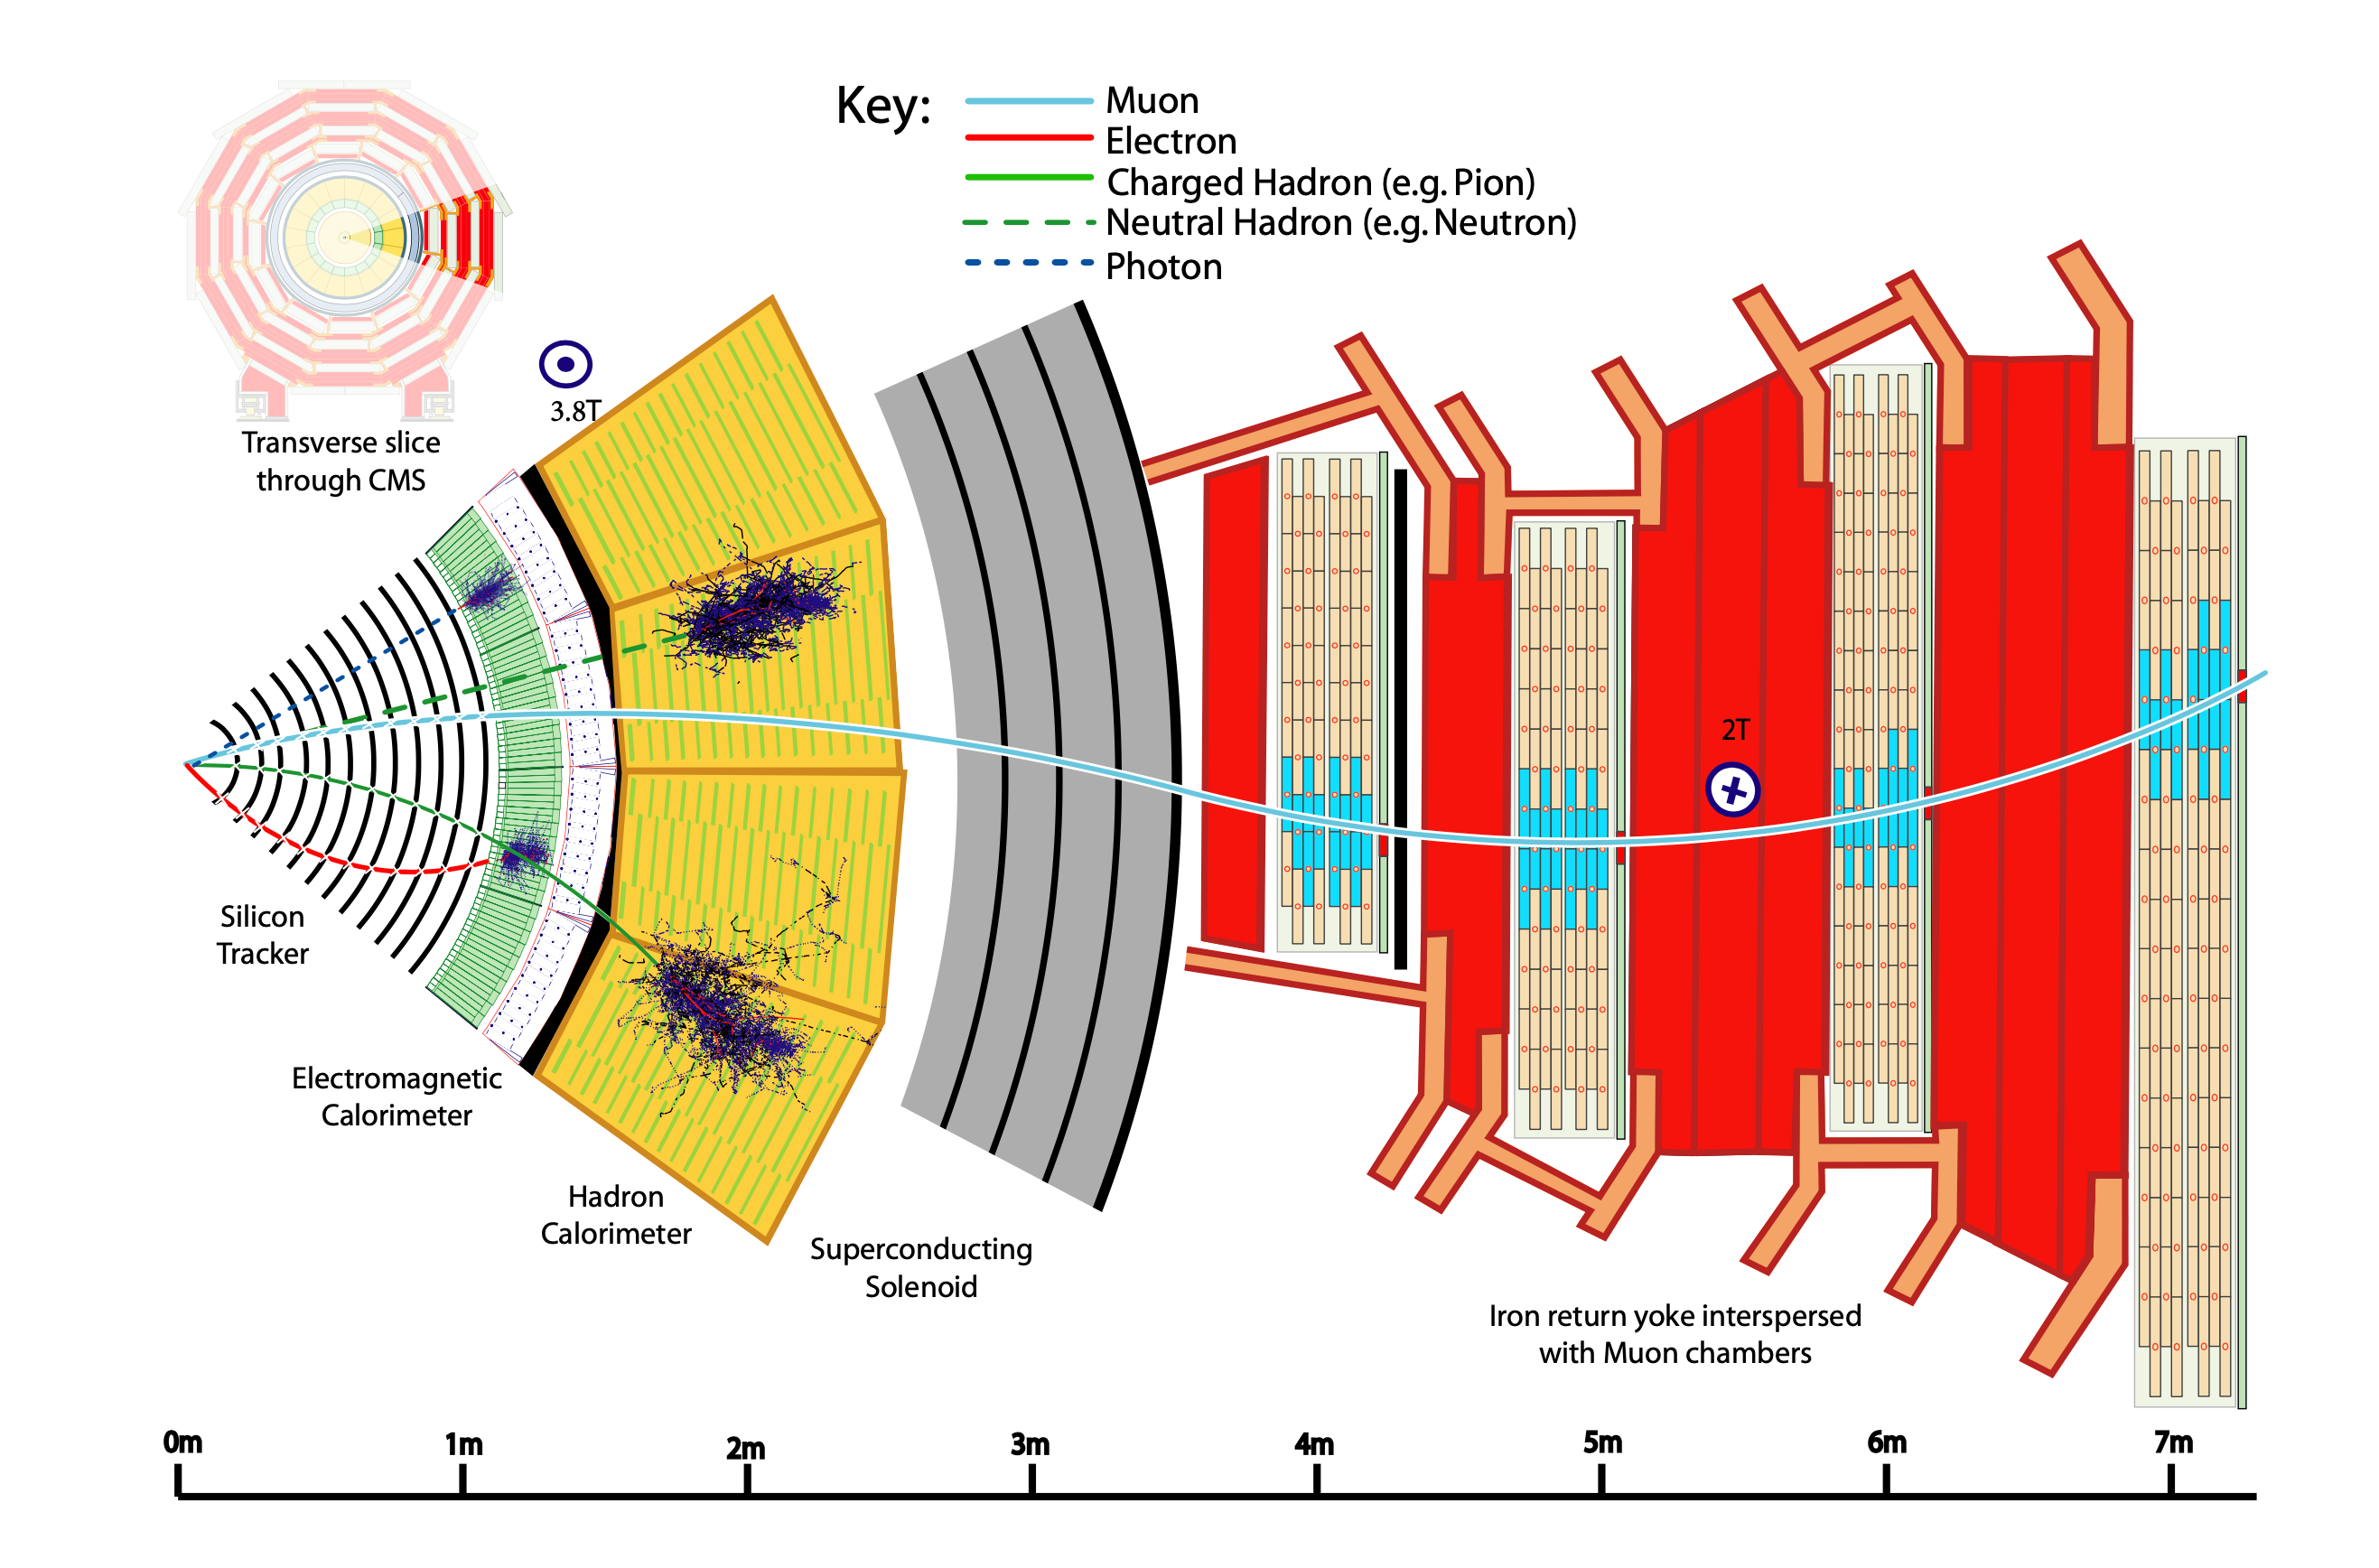
\includegraphics[width=0.8\textwidth]{chapters/CMSExperiment/sectionReconstruction/figures/pfa.png}
    \caption{The behaviors of different kinds of particle-flow candidates in the detector.}
    \label{fig:cmsExperiment:reconstruction:pfa}
\end{figure}

% different behaviors of pf candidates
Fig~\ref{fig:cmsExperiment:reconstruction:pfa} illustrates the behaviors of different kinds of particle-flow candidates in the detector. Starting from the beam interaction region, particles first enter the tracker, where the charged-particles leave trajectories while neutral particles do not. The tracker is immersed in a magnetic field that bends the trajectories. Electrons and photons are then absorbed in the ECAL. The corresponding electromagnetic showers are detected as clusters of energy depositions. Charged and neutral hadrons may initiate showers in the ECAL as well, which are subsequently fully absorbed in the HCAL. The corresponding clusters are used to estimate their energies and directions. Muons and neutrinos traverse the calorimeters with little or no interactions. While neutrinos escape undetected, muons produce tracks in the muon detector located outside the solenoid. So, muons are characterized by the tracks in the tracker and muon detector with MIP in ECAL and HCAL. Electrons and photons deposit energy in the ECAL with and without track correspondence, respectively. Charged and neutral hadrons deposit energy in both ECAL and HCAL with and without track correspondence, respectively. 


% pfa algorithm process
Regarding the algorithm process, the FPA begins with computing particle-flow elements in each subdetector, involving tracks in the tracker and the muon detector, clusters in the ECAL and the HCAL. Then PF elements in different subdetectors are linked to create PF Blocks via a linking process, such that a PF Block summarizes the activities of a potential particle candidate in all subdetectors. The details of reconstruction and linking of the PF elements can be found in \cite{cms:particleflow:Sirunyan:2017ulk}. In the end, PF candidates are identified from the PF blocks. PFA combines information from the entire detector to achieve the best possible energy resolution and particle identification, significantly outperforming the standalone reconstruction of individual subdetectors.




\subsection{Muon}
\label{sec:cmsExperiment:reconstruction:muon}

The reconstruction of muon involves a standalone reconstruction in the muon detector followed by a global reconstruction which combines the trajectories in the tracker. 

% standalone reco in muon chamber
The standalone reconstruction starts with the track segments in the individual muon chambers. The state vectors (track position, momentum, and direction) associated with the segments found in the innermost chambers are used to seed the muon trajectories, working from inside out, using the Kalman Filter (KF) technique \cite{tech:kf:Fruhwirth:1987fm}. The track parameters and the corresponding errors are updated at each step. The procedure is iterated until the outermost measurement surface of the muon system is reached. A backward Kalman-filter is then applied, working from outside-in. Finally, the track is extrapolated to the nominal interaction point, and a vertex-constrained fit to the track parameters is performed.

% global recon
The global muon reconstruction involves extending the muon trajectories to include hits in the silicon tracker. Starting from a standalone reconstructed muon, the trajectory is extrapolated from the innermost muon station to the outer tracker surface, taking into account the muon energy loss in the material and the effect of multiple scattering. This extrapolation and the associated uncertainty defines a region of interest in the tracker, where tracks are seeded by hit doublets and reconstructed using Kalman-filter. A final trajectory fit to the global hits is carried out to exact the muon momentum and impact parameters. This retains both prompt muons and muons from displaced vertices with the best possible efficiency and resolution. Figure~\ref{fig:cmsExperiment:reconstruction:resMu} shows the resolution of muon transverse momentum as a function of eta at different muon energies. The left plot is the result of the standalone reconstruction algorithm. The right is from the global reconstruction algorithm. A significant improvement is achieved when going from standalone to global muon reconstruction.

\begin{figure}[ht]
    \centering
    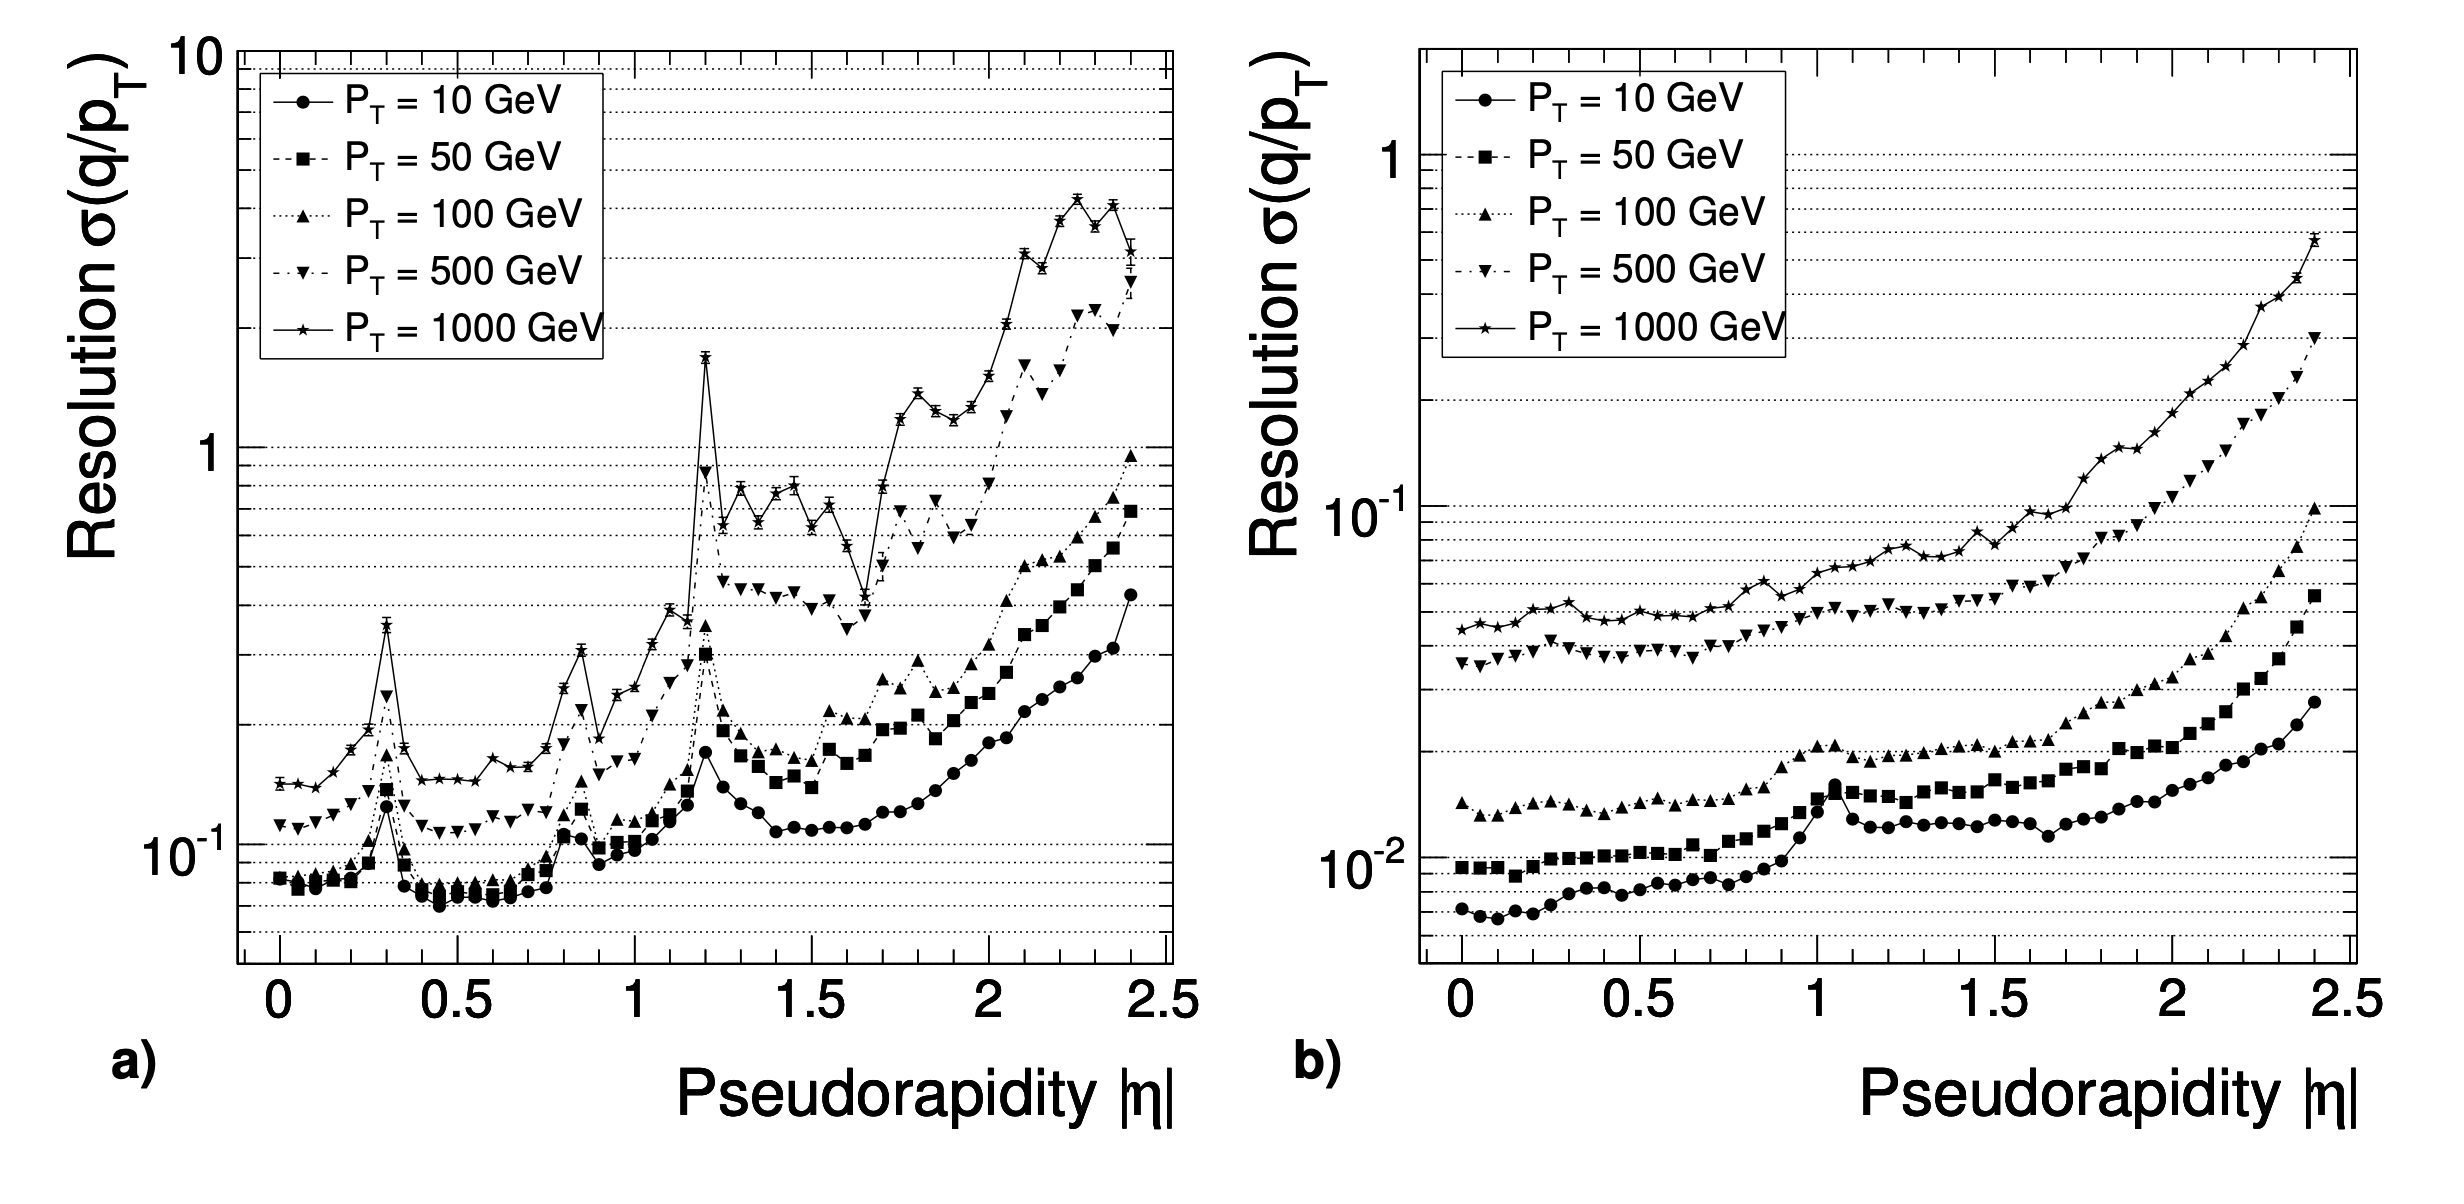
\includegraphics[width=0.95\textwidth]{chapters/CMSExperiment/sectionReconstruction/figures/resMu.png}
    \caption{The resolution of muon transverse momentum as a function of eta with different muon energies \cite{cms:tdr1:Bayatian:2006nff} . The left and right plots show the result of the standalone and global reconstruction, respectively.}
    \label{fig:cmsExperiment:reconstruction:resMu}
\end{figure}





\subsection{Electron and Photon}
\label{sec:cmsExperiment:reconstruction:egamma}


\begin{figure}[ht]
    \centering
    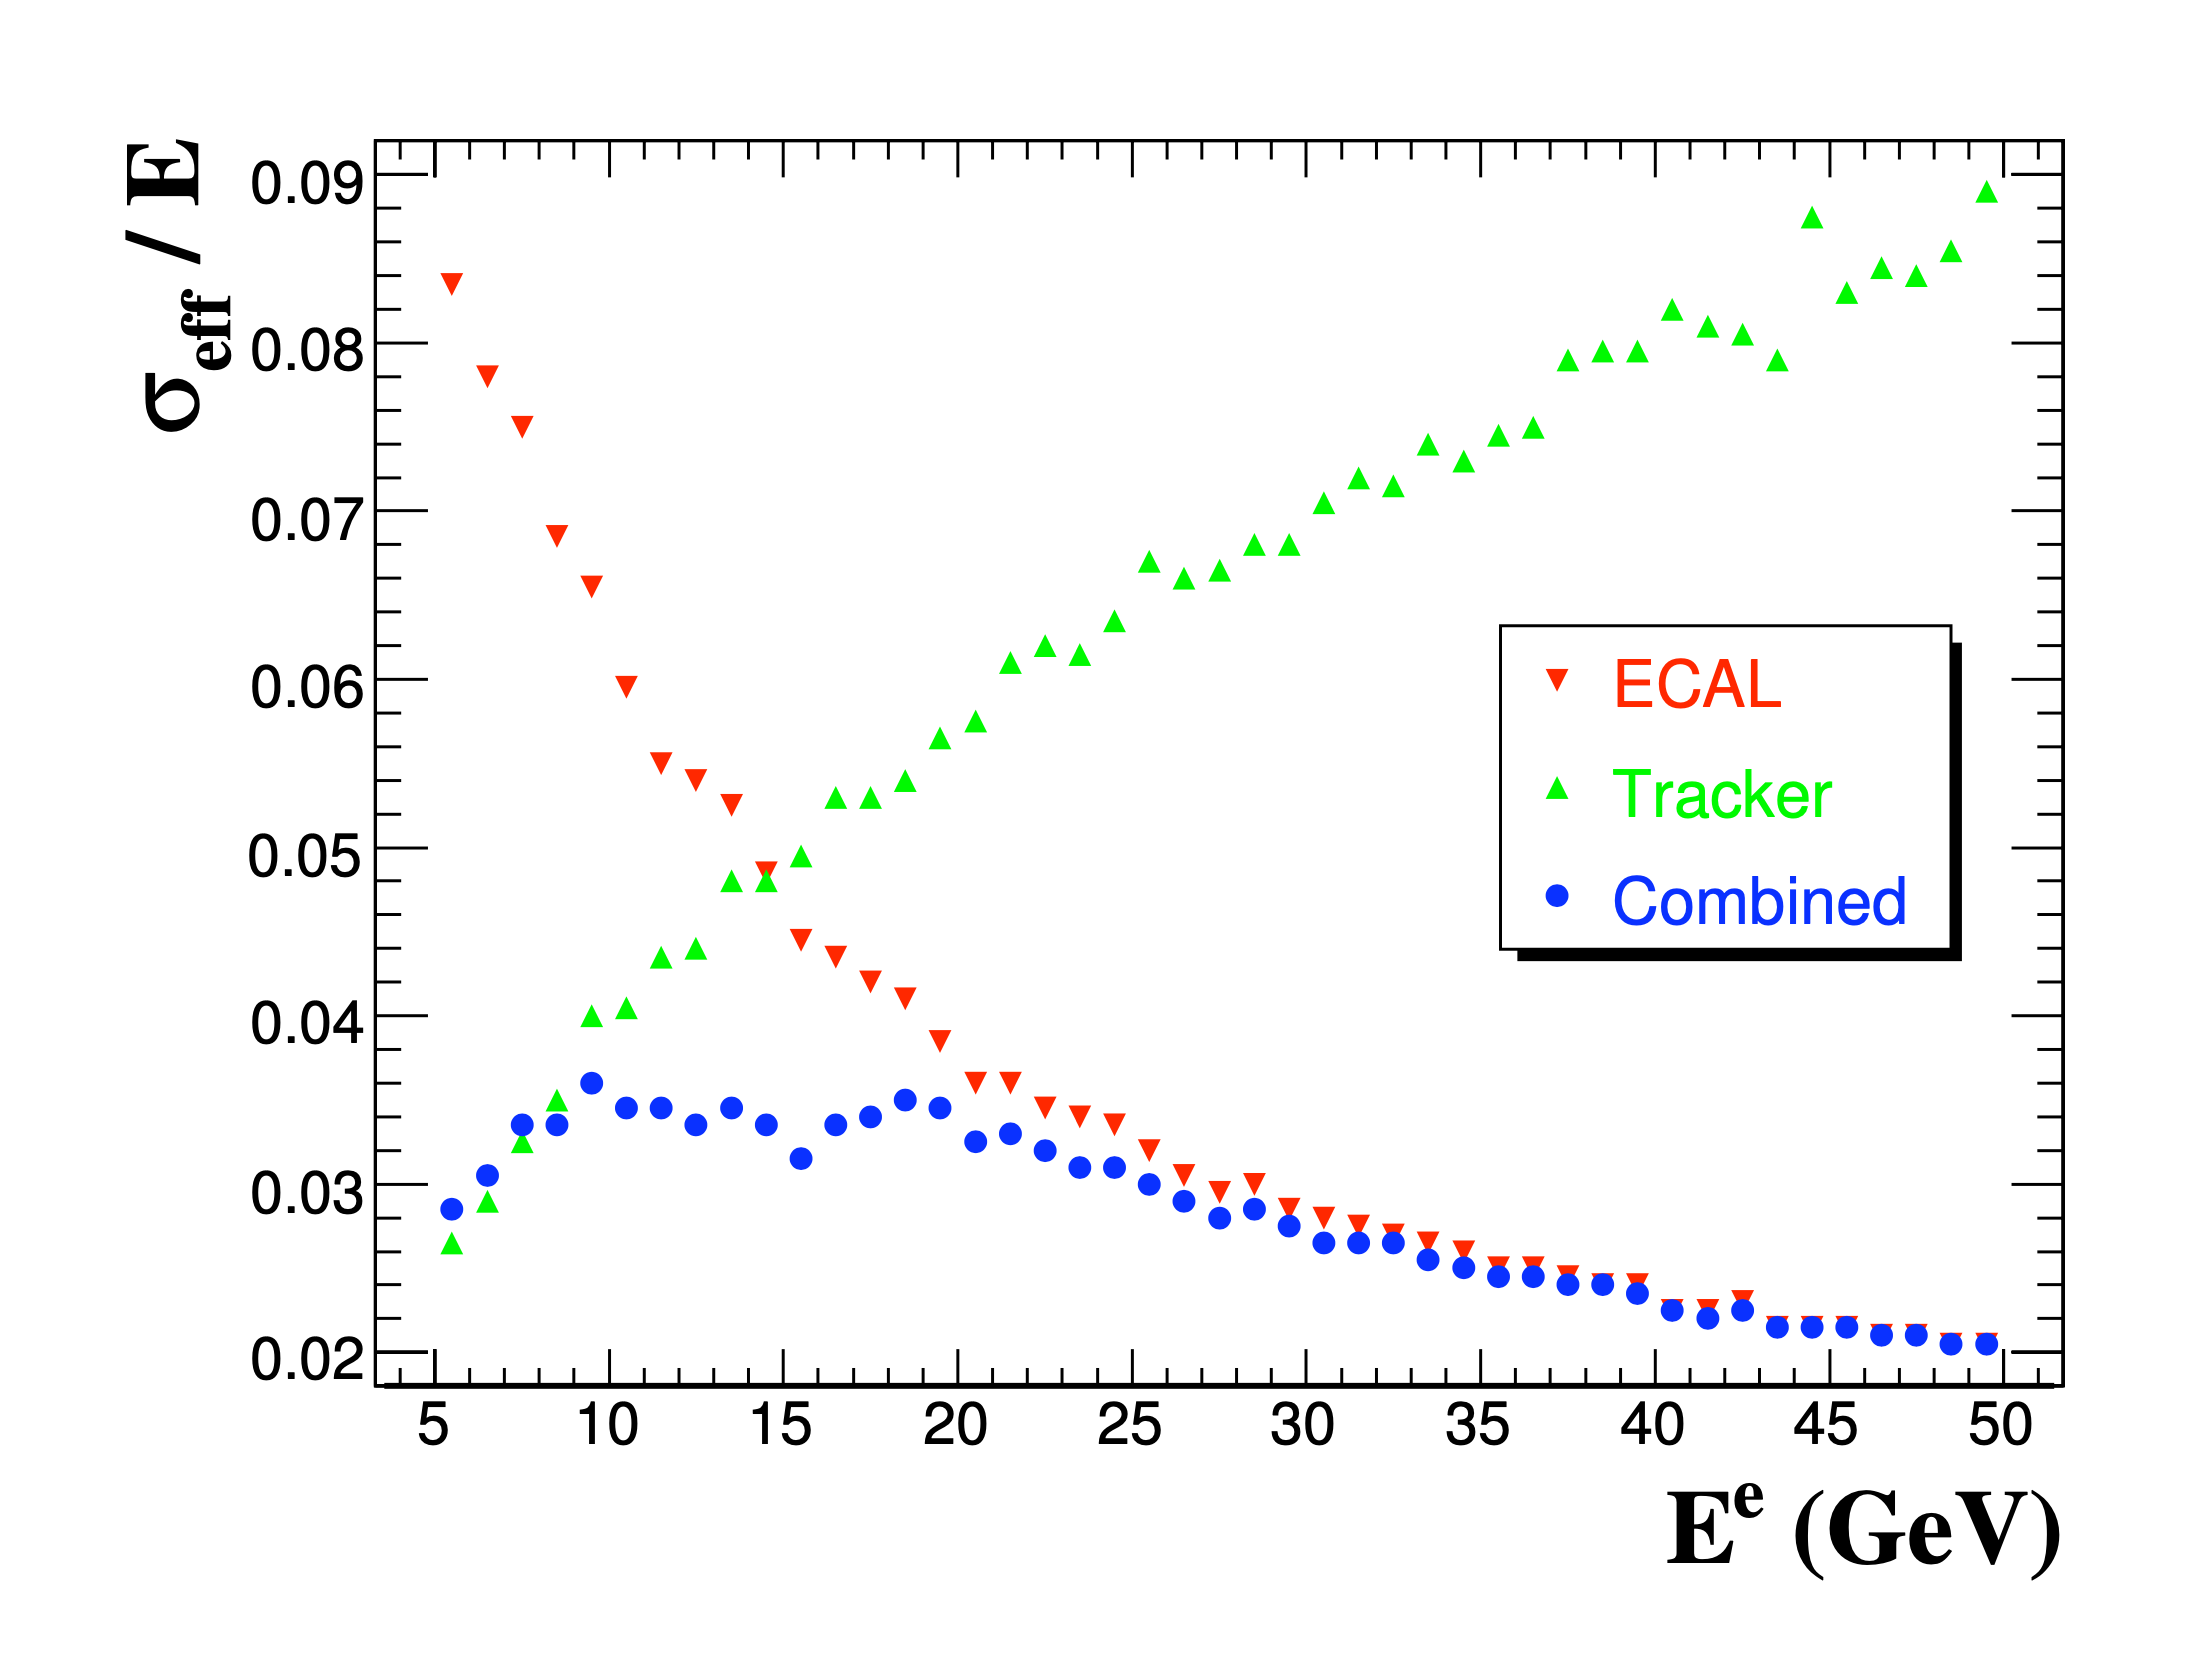
\includegraphics[width=0.5\textwidth]{chapters/CMSExperiment/sectionReconstruction/figures/resEle.png}
    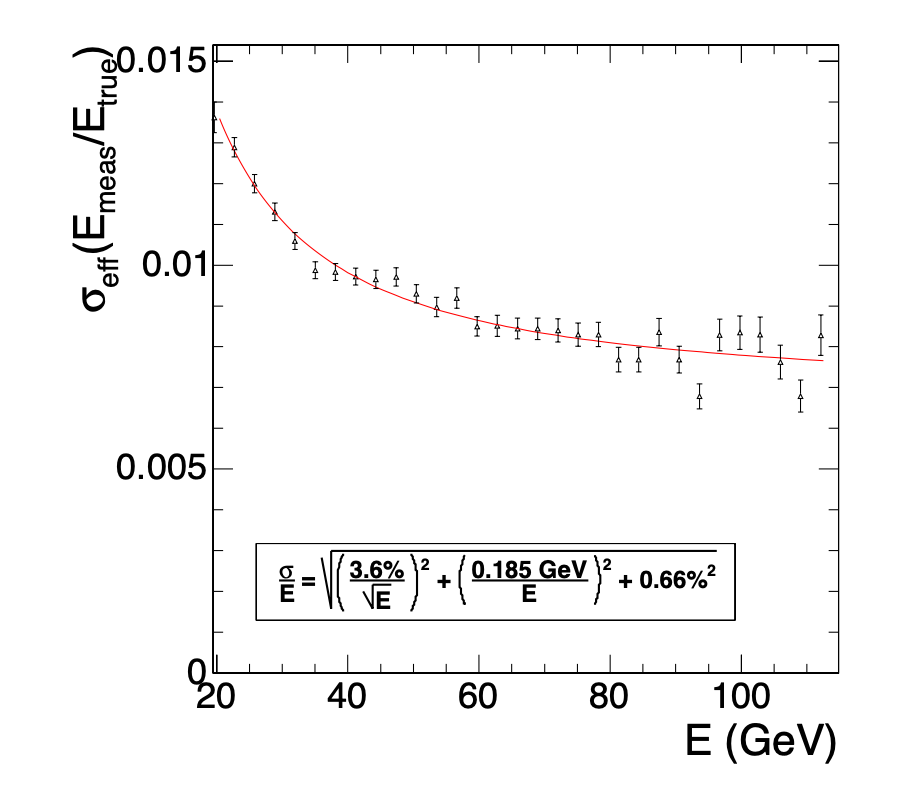
\includegraphics[width=0.42\textwidth]{chapters/CMSExperiment/sectionReconstruction/figures/resGamma.png}
    \caption{The energy resolution of the electron \emph{(left)} and photon \emph{(right)} \cite{cms:tdr1:Bayatian:2006nff}.  }
    \label{fig:cmsExperiment:reconstruction:resEle}
\end{figure}

% e-gamma conversion in tracker
The electron reconstruction in CMS is hampered by the amount of tracker material in front of the ECAL. The tracker material thickness varies strongly with $\eta$, as shown in Figure~\ref{fig:cmsExperiment:detector:trackerMaterial}. When electrons traverse the tracker's silicon layers, they radiate collections of bremsstrahlung photons, and thereby the energy reaching the ECAL spreads alone the $\phi$ direction. \cite{cms:tdr1:Bayatian:2006nff} provides a good illustration -- ''For electrons at $p^T=10~\GeV$, about half of the electrons radiate away more than half of their energy before reaching the surface of the ECAL. In about $10\%$ of the cases, more than $95\%$ of the initial electron energy is radiated!'' Furthermore, the radiated photon can again convert into electron-positron pairs, usually soft and trapped in the magnetic field, losing all the energy in the end undetected.

% reco of e and photon
The reconstruction of electron starts with making superclusters from the ECAL energy deposits. The superclustering algorithm is optimized for the scenarios of energy spread alone $\phi$ direction. The supercluster helps the finding of track seeds, which are hit doublets in the pixel detector. If a seed compatible with the supercluster is found, the track building begins inside-out with a nonlinear filter called Gaussian Sum Filter (GSF) \cite{tech:gsf:Adam:2005bya}. For superclusters successfully linked with GFS tracks, an electron candidate is made. A fit to the GSF tracks and ECAL superclusters is used to extract the four-momentum under the electron assumption. This combines the advantages of the tracker in the low energy region and the ECAL in the high energy region. The energy resolution of electrons using tracker-only, ECAL-only and the combined is shown in Figure~\ref{fig:cmsExperiment:reconstruction:resEle} (left). For a supercluster not linked to any GFS tracks, a photon candidate is made. The energy is obtained from the sum of energy deposited in a supercluster of crystals. To quantify the photon shower's lateral spread, a variable called R9 is defined for the supercluster. It equals to the 3x3 crystals' energy around the leading crystal divided by the total supercluster energy. It is used as a quantity for photon identification. The energy resolution of photons with R9 >0.943 is shown in Figure~\ref{fig:cmsExperiment:reconstruction:resEle} (right).



\subsection{Hadron}
\label{sec:cmsExperiment:reconstruction:hadron}

% nuetral hadron
Once muons, electrons, and isolated photons are identified, the remaining particles are neutral and charged hadrons. The calorimeter clusters not linked to any tracks suggest the non-isolated photons and neutral hadrons. Within the tracker acceptance ($|\eta|< 2.5$), all such ECAL clusters are turned into non-isolated photons, and all such HCAL clusters are turned into neutral hadrons. 

% changed hadron
Then the charged hadron reconstruction becomes the last step. Charge hadrons are made from the remaining calorimeter clusters and tracks. Each of the remaining HCAL clusters is linked to one or several tracks, which may in turn also link to some of the remaining ECAL clusters. It is possible that these remaining calorimeter clusters contain not only the charged hadrons but also the unresolved FSR photons and close-by non-isolated neutral hadrons around the charged hadrons. To identify these unresolved neutral components, a match of calorimeter energy and tracker momentum is carried out:

\begin{itemize}
    \item If the calorimetric energy is compatible with the linked track momenta, no neutral particle is identified. The charged hadron's kinematics are redefined by a global calibration taking into account both the tracker and the calorimeters. 
    \item If the calorimetric energy excesses the sum of the tracks momenta by an amount larger than the expected calorimetric energy resolution for hadrons, the excess may be interpreted as the presence of near-by photons and neutral hadrons. Such excess energy is in priority treated as a non-isolated photon and subtracted from the ECAL energy. In the case that the ECAL energy alone is not enough to account for the excess, the remaining excess is treated as a non-isolated neutral hadron. 
    \item If the calibrated calorimeter energy is smaller than the tracking momentum, an additional search for non-isolated muon is carried out with a relaxed muon reconstruction standard. The momentum of the looser reconstructed muons is then subtracted before a re-compare.
\end{itemize}







\subsection{Jet}
\label{sec:cmsExperiment:reconstruction:jet}


\begin{figure}[ht]
    \centering
    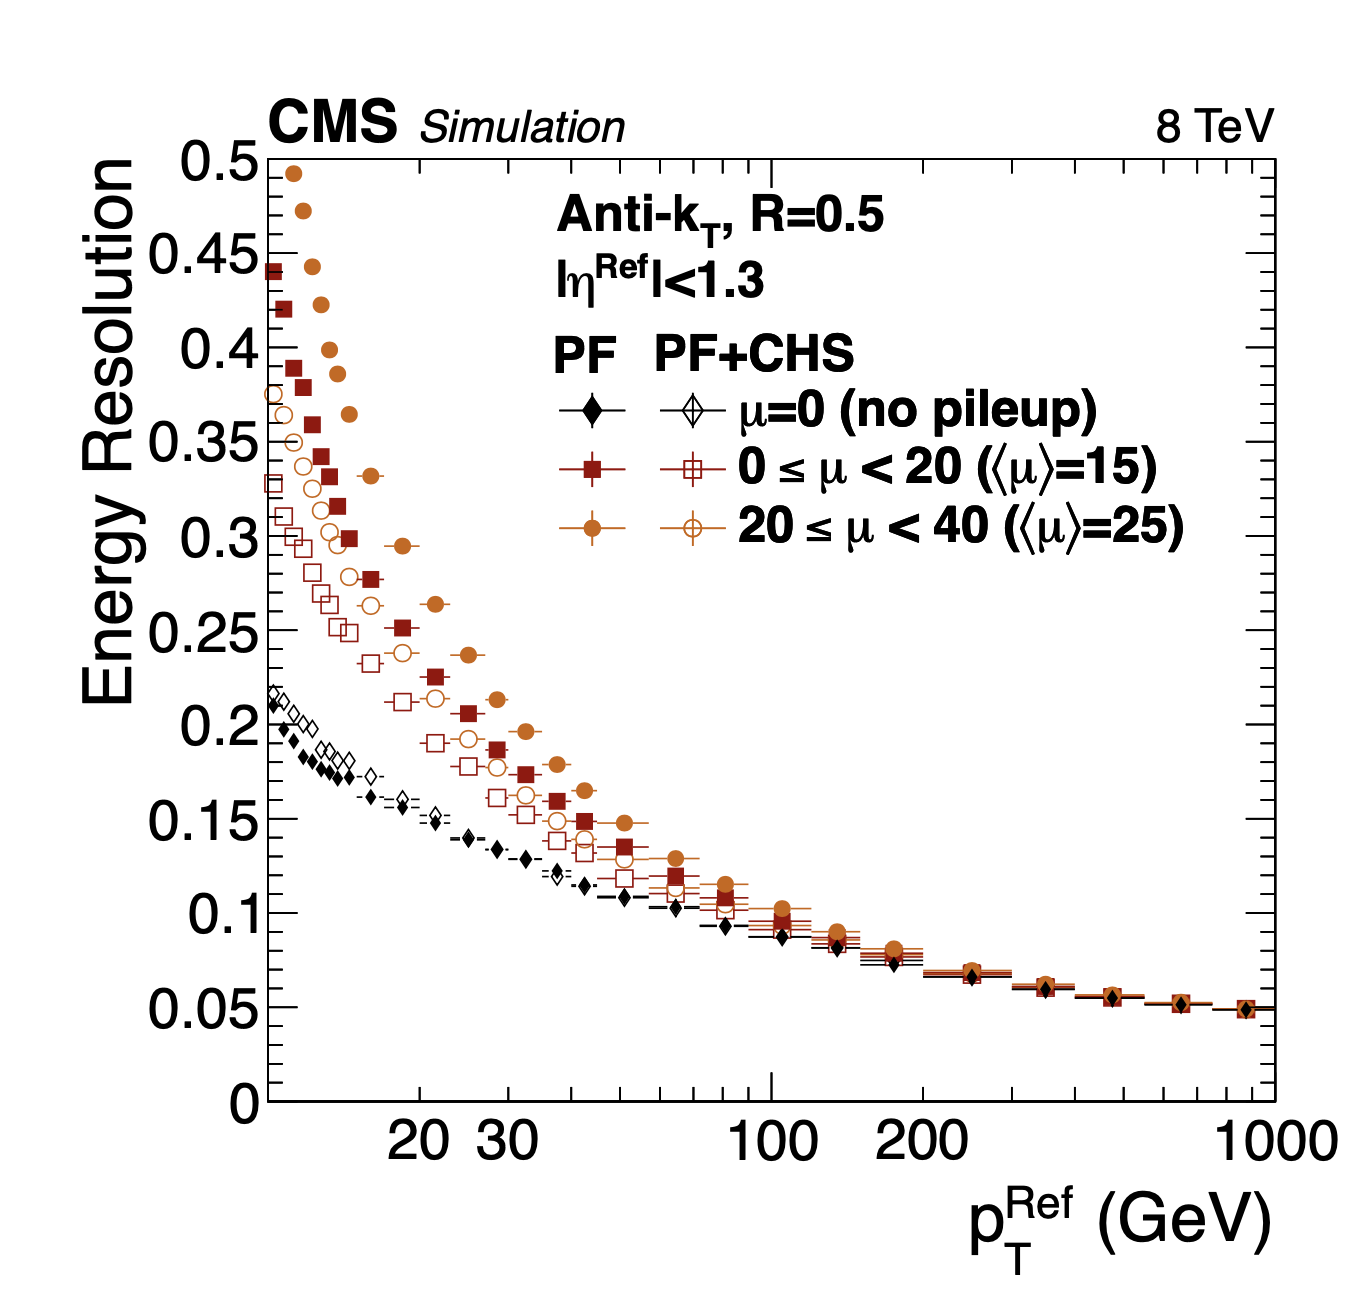
\includegraphics[width=0.5\textwidth]{chapters/CMSExperiment/sectionReconstruction/figures/jetres_pf_chs}
    \caption{ The jet energy resolution \cite{cms:particleflow:Sirunyan:2017ulk} with and without Charged Hadron Subtraction (CHS) in three pileup scenarios $\langle \mu\rangle =0,15,25$. The improvement from CHS is more prominent at higher pile-ups.  }
    \label{fig:cmsExperiment:reconstruction:resJet}
\end{figure}



% anti kt
With the PF candidates reconstructed, including muons, electrons, photons, charged and neutral hadrons, jets are produced by a clustering algorithm that groups colinear PF candidates to represent the particle originating from the hard process. The popular jet clustering algorithms include \kt, anti-\kt and Cambridge/Aachen algorithm \cite{tech:antikt:Cacciari:2008gp}, among which the key difference lies with the definitions of the distances. More specifically, if we denote the distance between two objects $i$ and $j$ as $d_{ij}$, the distance between the object $i$ and the beam as $d_i$,  the general form of the distances $d_{ij}$ and $d_i$ can be written as
\begin{equation}
	d_{ij} = \min(k^{2p} _{\mathrm{T},i}, k^{2p}_{\mathrm{T},j}) \; \frac{(\eta_i-\eta_j) ^2 + (\phi_i-\phi_j) ^2}{R^2} , \quad d_i =k^{2p} _{\mathrm{T},i},
\end{equation}
\noindent where $R$ is a algorithm parameter related to the cone size of the jets and $p$ is the power of $\kt^2$. The  \kt, anti- \kt and Cambridge/Aachen algorithm adopt $p=\{1,-1,0\}$, respectively. The clustering algorithm used in the CMS is the anti- \kt algorithm. The parameter $R$ is set to be 0.4 for slim jets and 0.8 for fat jets. During the anti- \kt clustering process, the shortest distance is searched among all the $d_{ij}$ and $d_i$ in the collection of PF candidates. If the minimal distance is $d_{ij}$, the two object $i$ and $j$ are merged into a new object. Otherwise, the minimal distance is $d_{i}$ and the object $i$ is output as a jet. This process is repeated until all objects are output. 

% charge hadron subtractionb#
The PF candidates in a jet may include the hadrons from the pile-up activities. The pile-up constituents in a jet become more relatively significant for the low \pt in the barrel region \cite{cms:particleflow:Sirunyan:2017ulk}. Hence a pile-up subtraction is designed to clean up the PF candidates from the pile-up. It removes charged hadrons not associated with the primary vertex. This step is called Charged Hadron Subtraction (CHS). Figure~\ref{fig:cmsExperiment:reconstruction:resJet} shows the jet energy resolution with and without CHS for three pileup scenarios $\langle \mu\rangle =0,15,25$. As the pile-up increases, the improvement from the CHS becomes more significant.  





\subsection{b Jet Tagging}
\label{sec:cmsExperiment:reconstruction:btag}

To identify the jets originating from the \PQb quarks, several tagging algorithms have been developed \cite{Chatrchyan:2012jua, Sirunyan:2017ezt, Bols:2020bkb}. 

The first tagger is Jet Probability (JP) and Jet B Probability (JBP). JP computes the likelihood for each track to come from the primary vertex, given the track's impact parameter and the spatial resolution of the primary vertex. Such likelihoods for all tracks in the jet are combined to indicate the probability of the jet coming from a non-prompt particle. JBP is a variation of JP. JBP assigns larger weights to the four tracks with the largest impact parameter. 

The second tagger is Combined Secondary Vertex (CSV). Compared with JP/JBP, which focuses on tracks' impact parameters, CSV also performs a searching and fitting for tracks' secondary vertices. Then, it computes several kinematic and topology variables about the secondary vertices, such as the number of SV, the distance of SV, the corrected SV mass, the relative SV energy ratio, and the number of tracks in the SV. The full list of the input variables of the CSV version-1 and version-2 used during the LHC run-1 and run-2 can be found in \cite{Sirunyan:2017ezt}. Finally, all the jet and jet's secondary vertex variables are fed into a multivariate model to obtain a single \PQb tag score. In the full run-2 dataset, with the same set of jet and jet's SV variables, the multivariate model is improved by a more flexible classifier, a fully-connected neural network (nn) with a few hidden layers. This nn-based tagger is called DeepCSV \cite{Bols:2020bkb}.

The third tagger is the combined multivariate analysis (cMVA). When electrons and muons present in a jet, the information related to the charged lepton is used to construct a soft-electron (SE) tagger and a soft-muon (SM) tagger, which are both boosted decision trees (BDT) trained with 2D and 3D lepton impact parameters and a few kinematic variables about the lepton's angular separation and relative \kt. Then an MVA combines the JP, JBP, CSV, SE, SM taggers into a final comprehensive \PQb tag score. Figure~\ref{fig:cmsExperiment:reconstruction:cMVA} shows the distributions of the \PQb tag score from the cMVA \PQb tagger for the simulated light, c and \PQb jets.

\begin{figure}[ht]
    \centering
    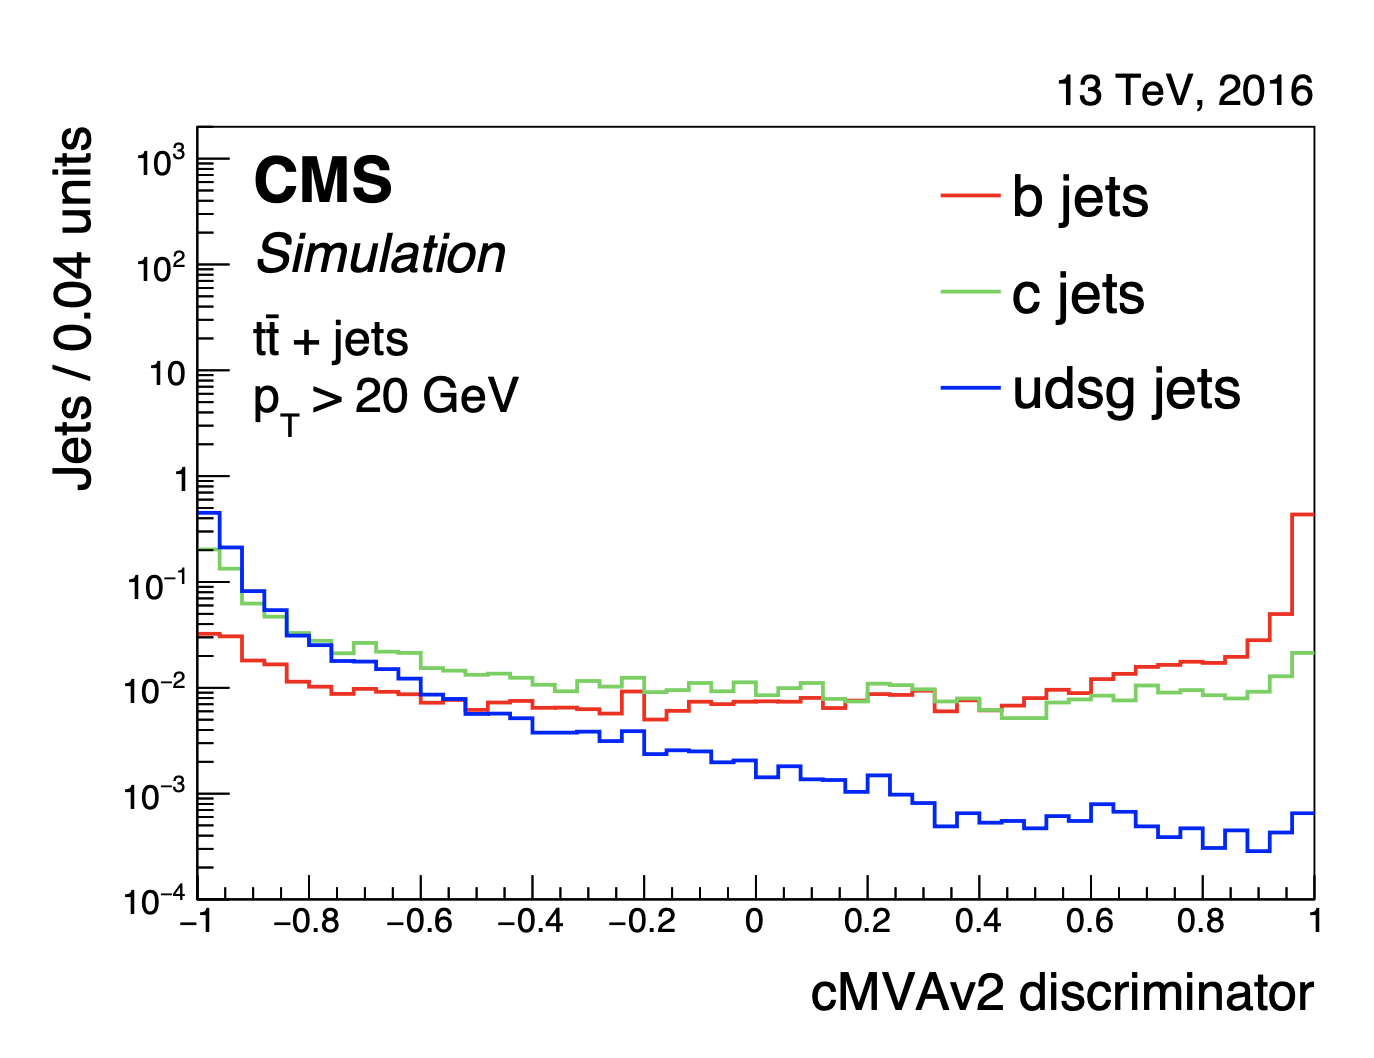
\includegraphics[width=0.5\textwidth]{chapters/CMSExperiment/sectionReconstruction/figures/cMVA}
    \caption{The distribution of the \PQb tag score from the combined multivariate analysis (cMVA) \PQb tagger \cite{Sirunyan:2017ezt}. }
    \label{fig:cmsExperiment:reconstruction:cMVA}
\end{figure}





\subsection{Hadronic Tau Identification}
\label{sec:cmsExperiment:reconstruction:tau}

About $64.8\%$ of taus decay hadronically. The major decay modes of hadronic taus include $B(\PGt^- \to h^- \PGnGt)=11.5\% $, $B(\PGt^- \to h^- \PGp^0 \PGnGt)=25.9\% $ (where the mass of $h^-\PGp^0$ system is resonant at $\rho(770)$), $B(\PGt^- \to h^- \PGp^0 \PGp^0 \PGnGt)=9.5\% $ and $B(\PGt^- \to h^- h^+ h^- \PGnGt)=9.8\% $ (where mass of $h^- \PGp^0 \PGp^0$ and $h^- h^+ h^- $ system is resonant at $a_1(1260)$). The tau reconstruction at the CMS relies on these hadronic decay modes.

For each reconstructed jet, the tau reconstruction first attempts to match the jet constituents to the patterns of the common hadronic decay modes. The matching, also known as mode finding, is performed with the hadrons-plus-strips (HPS) algorithm. If the jet structure is found compatible with a decay mode and the decay mode involves certain meson resonances like $\rho(770)$ and $a_1(1260)$, HPS further checks consistency between visible mass of the tau candidate and the expected meson resonance. After the mode finding, a $\PGth$ score based on the structure and isolation of the candidate's constituents is computed to discriminate against fakes from the quark or gluon jets, which could otherwise be significant due to the complex QCD environment in the LHC. Besides, discriminators against the electron and muon are also developed.


\subsubsection{The $\PGth$ Mode Finding}

Starting from the constituents of the reconstructed jets, the hadrons-plus-strips (HPS) algorithm is used to match the jet structure to the expected $\PGth$ pattern. 

% strip clustering: seeding-merging
The $\PGp^0$ mesons from the $\PGth$ decay promptly decay into pairs of photons, which are highly likely to convert into $ \Pe+ \Pe-$ pairs as they traverse the tracker material. The CMS magnetic field bends the $ \Pe+ \Pe-$ and leads to a spatial separation of the e+e− pairs on the $\eta-\phi$ plane. The electron and photon candidates within a certain region of $\Delta\eta \times \Delta \phi$  are clustered together to reconstruct the neutral pions. The resulting cluster is referred to as a “strip”. The strip's four-momentum is defined as the sum of all its constituent four-momenta. The clustering process defines a $\Delta\eta \times \Delta \phi = 0.20\pt^{-0.66} \times 0.35 \pt^{-0.71}$ window for each of the strips, electrons, photons. The steps of the strip clustering process work as follows: the leading $ \Pe/\PGg$ in the jet not yet included in any strips is used to seed a new strip; then, in order of deceasing \pt, the nearby $ \Pe/\PGg$ whose window touches the strip window is merged with the strip, and the strip's position and four-momentum are updated accordingly. These two steps of seeding and merging are repeated until all qualified $ \Pe/\PGg$ are processed. Comparing with a fixed window size employed during the run-1, the window size of this strip clustering algorithm depends dynamically on the object's \pt and better accounts for the different bending effects of different \pt.

% prong
Charged particles, often called prong, used in the reconstruction of $\PGth$ candidates are required to have $\pt>0.5$ GeV and must be compatible with the primary vertex. Due to the tau lifetime, when imposing primary vertex association, the transverse impact parameter is relaxed to $d_{xy}<0.1$~cm. The requirement of $\pt > 0.5~\GeV$ on the charged particles ensures that the corresponding tracks have sufficient quality.

% mode finding and mass constrain
Based on the reconstructed strips and qualified tracks in a jet, the HPS algorithm generates all possible combinations of hadrons for the following decay modes: $h^\pm$, $h^\pm \PGp^0$, $h^\pm \PGp^0 \PGp^0$, $h^\pm h^\mp h^\pm$. For $h^\pm \PGp^0$ decay mode, the total hadronic elements should be from $\rho(770)$ resonance. For $h^\pm \PGp^0 \PGp^0$ and $h^\pm h^\mp h^\pm$, the total hadronic elements should be from $a_1(1260)$ resonance. So if $h^\pm \PGp^0$ or $h^\pm \PGp^0 \PGp^0$ or $h^\pm h^\mp h^\pm$ mode is found, the total visible mass of the tau candidate is checked to be compatible with corresponding resonance. Last but not least, for each $\PGth$ candidate, a signal cone is defined as
\begin{equation}
	\Delta R_{sig} = \frac{3.0 \text{ GeV } } { \pt (\text{ hadronic system})  }, \quad \text{with } 0.05 \leq \Delta R_{sig} \leq 0.1.
	\label{eqn:cmsExperiment:reconstruction:tauSigRegion}
\end{equation}

\noindent If any charged particles or strip is located outside the signal cone, the $\PGth$ candidate is rejected.

\subsubsection{Discriminator against jets}

To reduce the fakes from gluon or quark jets, discriminators are designed against $j\to \PGt$ fakes for the $\PGth$ candidates. Comparing with the quark and gluon jets, the $\PGth$ tends to have a cleaner calorimeter environment in its near-by region. Base on this principle, an isolation quantity in a $\Delta R = 0.3$ cone is calculated. Two discriminators have been developed for 2016 analysis. They are isolation sum discriminator and MVA-based discriminator. For Run-2, the MVA classifier is improved by a more flexible classifier model, deep neural networks. 

% iso based
The isolation of $\PGth$ candidate is computed by summing the \pt of charged particles and photons in a $\Delta R = 0.3$ cone around the $\PGth$ candidate. The summing does not include the charged particle and photons of the $\PGth$ candidate in the $tau_h$ signal cone defined in Equation~\ref{eqn:cmsExperiment:reconstruction:tauSigRegion}. The $\PGth$ isolation is defined as
\begin{equation}
	I_{\PGth} = \sum \pt^{\text{charged}} (d_z<0.2 \text{cm}) + \max \bigg( 0, \sum \pt^ \PGg - \Delta \beta \sum \pt^{\text{charged}} (d_z>0.2 \text{cm})  \bigg )
    \label{eqn:cmsExperiment:reconstruction:tauIso}
\end{equation}

\noindent where $d_z<0.2$~cm requirement reduces the PU contributions in the $\sum \pt^{\text{charged}}$. Meanwhile, PU contributions in the $\sum \pt^ \PGg $ is subtracted by the term $\Delta \beta \sum \pt^{\text{charged}} (d_z>0.2~\text{cm}) $, where the parameter $\Delta \beta =0.2$ scales the PU charged component to estimate the PU neutral component. The isolation sum discriminator requires $I_{\PGth} $ to be less than some working point. In addition to $I_{\PGth}$ cut, the \pt of the partial strip located outside the $\PGth$ signal cone, denoted as $\pt^{\text{strip, outer}} $, is calculated and requirement
\begin{equation}
    \pt^{\text{strip, outer}} < 0.1 \pt^{\PGth}
    \label{eqn:cmsExperiment:reconstruction:ptStripOuter}
\end{equation}

\noindent is imposed to further reduce $j \to \PGth$ fakes given that the strip window in the strip clustering is dynamically \pt dependent. This additional cut on $\pt^{\text{strip, outer}}$ approximately reduces $j \to \PGth$ fakes by another $20\%$ without impacting the $\PGth$ efficiency.


\begin{figure}[ht]
    \centering
    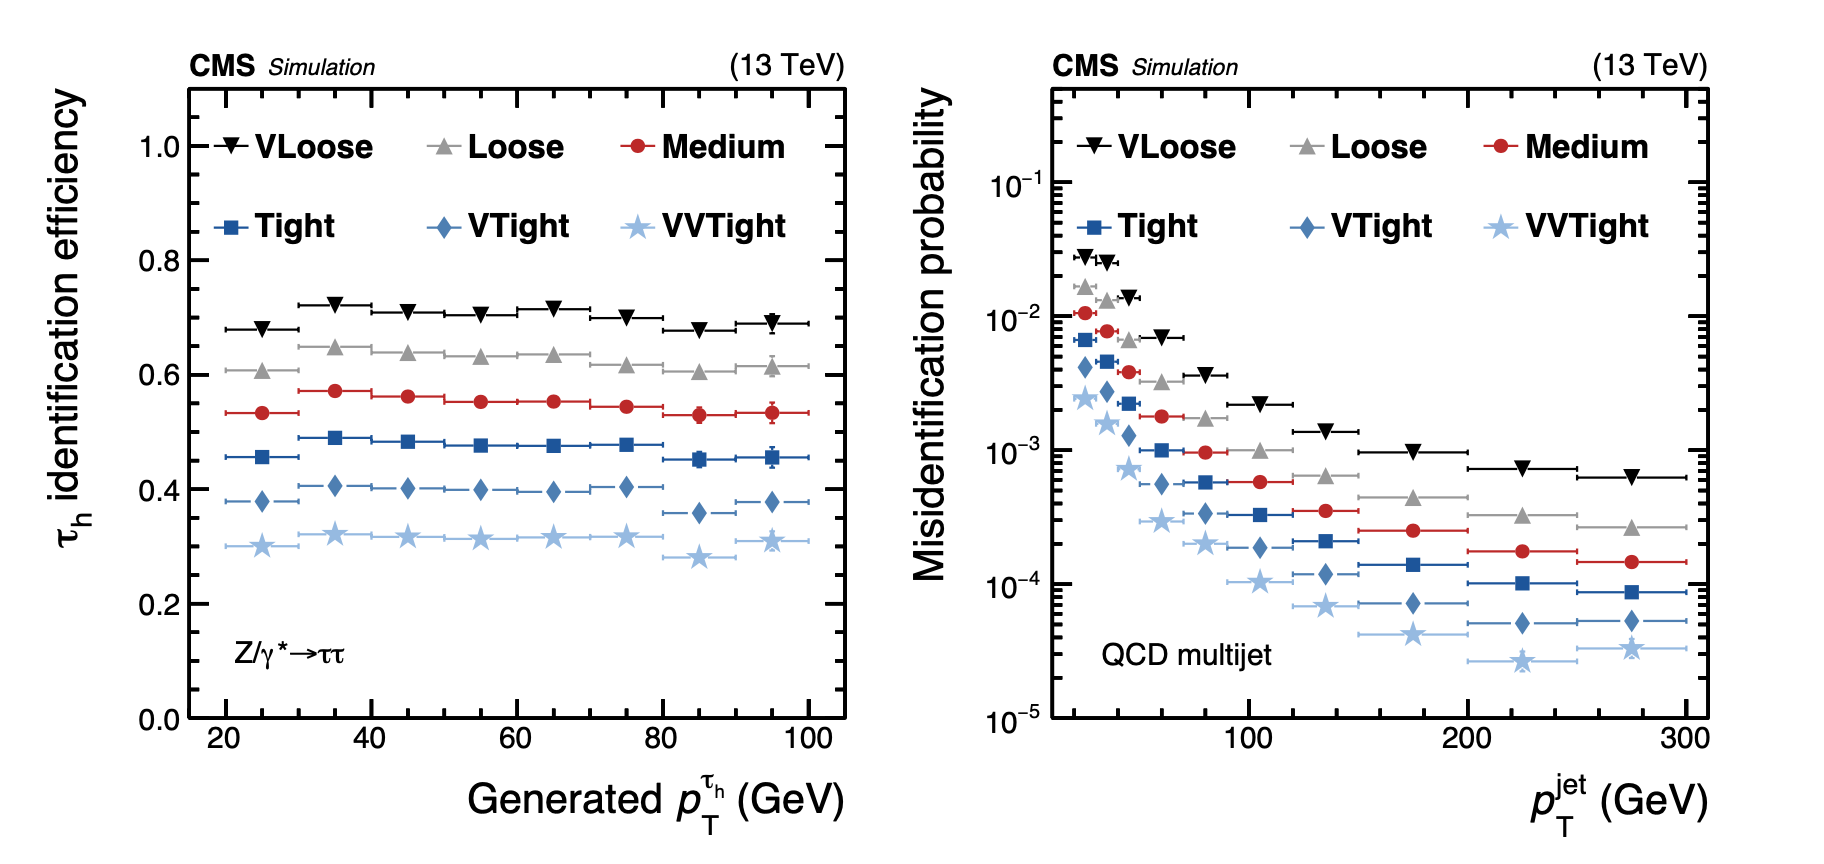
\includegraphics[width=0.9\textwidth]{chapters/CMSExperiment/sectionReconstruction/figures/tauMVA}
    \caption{ The $\PGth$ identification efficiency and $j\to \PGth$ misidentification probability in the QCD multijets events \cite{Sirunyan:2018pgf}. Different working points are shown in different colors. }
    \label{fig:cmsExperiment:reconstruction:tauMVA}
\end{figure}

% mva based


MVA-based $\PGth$ discriminator combines the isolation and other topology variables sensitive to the $\PGt$ lifetime \cite{Sirunyan:2018pgf} to provide the best possible discrimination between $\PGth$ and quark or gluon jets. The MVA classifier is a boosted decision tree (BDT). The input variables to the MVA includes $I_{\PGth}$ in Equantion~\ref{eqn:cmsExperiment:reconstruction:tauIso}, $ \pt^{\text{strip, outer}}$ in Equation~\ref{eqn:cmsExperiment:reconstruction:ptStripOuter}, spatial separations among $ \Pe/\PGg$ in the strips, significance of the 3D impact parameter (SIP3D) of the leading tracks, tau flight length for 3 prong $\PGth \to h^\pm h^\mp h^\pm$ calculated by the secondary vertices. The full list of the input variables can be found in \cite{Chatrchyan:2012zz, Khachatryan:2015dfa}. Based on the MVA result, the isolation variable provides the most discriminating power. The next important variables are SIP3D and tau flight length. The MVA combines all sensitive variables and outputs a single number for the $\PGth$ identification score, which can be cut at different working points. Using different MVA working points, the $\PGth$ identification efficiency and $j\to \PGth$ misidentification probability in the QCD multijets events are shown in Figure~\ref{fig:cmsExperiment:reconstruction:tauMVA}. The $\PGth$ identification is relatively constant with respective to \pt. In contrast, the misidentification probability drops significantly with the increase of \pt. 

In addition to the isolation discriminator and MVA-based discriminator, Deep Tau Identification is also developed for the Run-2 analysis. The deep tau ID is similar to the MVA-based ID in the sense of combining a set of sensitive variables to a single $\PGth$ score with a non-linear classification model. The difference is that the deep tau ID uses deep neural networks instead of BDTs for a more flexible classification. 





